\documentclass{article}
% 中文支持：仅保留 ctex（xeCJK 已内置，无需重复加载）
\usepackage[scheme=plain]{ctex}
\usepackage{parskip}
% \setlength{\parskip}{1em} % 段落间距设为 1 个字符宽度（推荐 0.8em~1.2em）
\setlength{\parindent}{0em} % 首行缩进保持 2 字符（中文排版默认，可选）
% 基础必备包（无冲突）
\usepackage[dvipsnames]{xcolor}
\usepackage[table]{xcolor} % 表格颜色支持
\usepackage{graphicx}       % 插入图片
\usepackage{float}          % 固定图片位置 [H]
\usepackage{caption}        % 优化图题/表题格式（与 subcaption 兼容）
% \usepackage{subcaption}     % 子图功能（替代 floatrow 的 subfloatrow）
% 参考文献相关
\usepackage{biblatex}
\addbibresource{references.bib}
% 辅助功能包
\providecommand{\tightlist}{%
  \setlength{\itemsep}{0pt}\setlength{\parskip}{0pt}}
\usepackage[utf8]{inputenc} % UTF-8 输入
\usepackage[T1]{fontenc}    % T1 字体编码
\usepackage{hyperref}       % 超链接
\usepackage{url}            % URL 排版
\usepackage{booktabs}       % 专业表格线
\usepackage{amsfonts}       % 数学符号
\usepackage{nicefrac}       % 分数符号
\usepackage[misc]{ifsym}    % 辅助符号
\usepackage{microtype}      % 微排版优化
\usepackage{xcolor}         % 颜色支持
\usepackage{enumitem}       % 列表环境优化
% 数学与表格相关
\usepackage{amsmath}
\usepackage{amssymb}
\usepackage{multirow}       % 表格跨行
\usepackage{makecell}       % 表格单元格换行
\usepackage{tabularx}       % 自适应宽度表格
\usepackage{xltabular}      % 长表格+自适应宽度
\usepackage{longtable}      % 跨页长表格
% 其他功能
\usepackage{framed}         % 带框文本
\usepackage{chngcntr}       % 计数器控制
\newenvironment{continueframe}{%
    \advance\linewidth-2\fboxsep
    \advance\linewidth-2\fboxrule
    \hsize=\linewidth
    \partialboxdim=\dimexpr\pagegoal-\pagetotal-\pageshrink-6pt-\baselineskip\relax
    \setbox\totalbox=\vbox\bgroup\begingroup
}{%
    \endgraf\endgroup\egroup
    \setbox\partialbox=\vsplit\totalbox to\partialboxdim
    \par\smallskip
    \hbox{\fbox{\vbox{\unvbox\partialbox}}}\nopagebreak
    % \par\smallskip\mbox{}\hfill\textbf{Continued on next page}\par\pagebreak%
    % \par\smallskip\mbox{} \par\pagebreak%
    
    % \hbox{\fbox{\vbox{\noindent\textbf{Continued from last page}\par\smallskip\unvbox\totalbox}}}%
    % \par\medskip
}

\newcommand{\down}[1]{\textcolor{PineGreen}{\small \ $\downarrow${#1}}}

\usepackage{geometry} % 控制页面边距、尺寸的核心包
% 格式：left=左边距, right=右边距, top=上边距, bottom=下边距
% 单位：cm 或 in（推荐 cm，更直观）
\geometry{left=2.0cm, right=2.0cm, top=2.5cm, bottom=2.5cm}
% 图题间距调整
\setlength{\belowcaptionskip}{-5pt}
\author{}
\begin{document}
    % \maketitle
    
\section{引言}\label{ux4e00ux5f15ux8a00}
随着人工智能技术的变革，单一模态的模型已经难以满足复杂场景下的交互需求，视觉-语言跨模态模型（LLM+Vision）成为业界研究和关注的核心方向。这类模型旨在融合视觉信息和语言信息，实现如图像描述、视觉问答、多模态对话等通用且复杂的任务。

BLIP-2、LLaVA与MiniGPT-4无疑是视觉-语言跨模态领域的代表性模型。尽管三者在模型架构的细节设计上各有侧重，但均采用了''视觉特征对齐-语言生成能力/多模态指令微调''的两阶段训练策略，为探索视觉与语言模型的深度融合提供了极具参考价值的技术范式。深入剖析这三大模型的技术路径可以发现，它们既面临着跨模态领域的共性核心问题，也在各自的优化方向上呈现出独特的技术思考。

它们共同面临的首要核心问题，是\textbf{模态鸿沟的跨越与特征表示的高效融合}。预训练视觉编码器(如ViT、CLIP)与大语言模型(如Flan-T5、Vicuna)是在完全不同的数据分布和任务目标下训练而成的：视觉编码器专注于提取图像的空间特征与视觉语义，输出的是高维密集特征向量；而大语言模型则擅长捕捉文本的序列依赖与语义关联，其输入为离散的token序列。如何设计高效的''桥梁模块''(如BLIP-2的Q-Former、LLaVA的线性投影层)来对齐和融合这两种截然不同的特征表示，是实现视觉-语言联合理解与生成的关键。

第二个共同挑战在于\textbf{轻量化高效训练策略的设计与成本控制}。由于大语言模型通常包含数十亿参数，直接联合训练会带来巨大的计算和存储开销。BLIP-2、LLaVA与MiniGPT-4均采用冻结预训练模型参数，仅训练连接模块和微调少量大语言模型的策略(LLaVA)，大幅降低了训练成本。同时，它们还通过精心设计的预训练任务(如图像-文本对比、匹配与生成)和微调数据集(如指令跟随数据)来提升模型在复杂多模态任务中的表现。

相较于BLIP-2更侧重于模型架构层面的特征融合创新，LLaVA与MiniGPT-4在实践中进一步关注到了\textbf{高质量微调数据对模型能力}(尤其是指令跟随能力/语言连贯性)的增益作用，这也成为两者区别于其他早期模型的重要技术特征。例如，LLaVA利用GPT-4生成了15万条视觉-语言指令对的数据集；MiniGPT-4则利用一阶段模型和GPT-4辅助生成了高质量多模态指令数据，进一步提升了模型在复杂视觉问答和多轮对话中的表现。这些实践充分证明，高质量、多样化的微调数据能够有效提升模型对复杂指令的理解能力、视觉细节的捕捉能力以及回答的准确性与逻辑性，是弥补模型''模态偏见''、提升交互自然度的重要支撑。

\section{核心技术对比}\label{ux4e8cux6838ux5fc3ux6280ux672fux5bf9ux6bd4}

% \begin{longtable}[]{@{}
%   >{\raggedright\arraybackslash}p{0.23\linewidth}  % 留足间距，避免溢出
%   >{\raggedright\arraybackslash}p{0.23\linewidth}
%   >{\raggedright\arraybackslash}p{0.23\linewidth}
%   >{\raggedright\arraybackslash}p{0.23\linewidth}@{}}
% \toprule
% \begin{minipage}[b]{\linewidth}\raggedright
% 对比维度
% \end{minipage} & \begin{minipage}[b]{\linewidth}\raggedright
% BLIP-2
% \end{minipage} & \begin{minipage}[b]{\linewidth}\raggedright
% LLaVA
% \end{minipage} & \begin{minipage}[b]{\linewidth}\raggedright
% MiniGPT-4
% \end{minipage} \\
% \midrule
% \endhead
% \bottomrule
% \endlastfoot
% \textbf{视觉编码器} & 冻结预训练ViT系列，支持ViT-L/14、ViT-g/14等 &
% LLaVA 1.0用CLIP ViT-L/14-224px；LLaVA 1.5\cite{liu2024improvedbaselinesvisualinstruction}升级为CLIP ViT-L/14-336px &
% 使用冻结的BLIP-2预训练组件(EVA-CLIP中的ViT-g/14 和 Q-Former) \\
% \textbf{大语言模型（LLM）} &
% 冻结开源LLM，如OPT（解码器）、Flan-T5（编解码器） & Vicuna7B(解码器) &
% 冻结的Vicuna等(解码器) \\
% \textbf{跨模态连接模块} & 轻量级Querying
% Transformer（Q-Former），含32个768维查询向量,
% 学习视觉-语言表征，再用线性层将查询向量映射成语言模型相同维度且作为软提示加入到LLM中
% & LLaVA 1.0用单一线性层；LLaVA 1.5升级为两层线性层+激活函数的MLP结构 &
% 冻结的Q-Former + 线性投影层 \\
% \textbf{核心训练数据集} & 预训练：COCO, Visual Genome, CC3M, CC12M,SBU,
% 115M from LAION-400M；（使用CapFilt方法创建人工注解） &
% 预训练：CC3M筛选的595K图像-文本对；微调：158K指令跟随数据 &
% 预训练：5M弱标注图像-文本对, 来自Conceptual Caption,
% SBU和LAION数据集；微调：3.5K高质量多模态指令数据；Localized
% Narratives数据集 \\
% \textbf{训练阶段划分} & 阶段一:
% 基于冻结视觉编码器的视觉-语言表示学习；阶段二:
% 基于冻结LLM的视觉-语言生成学习 & 阶段一:
% 特征对齐预训练（训投影层）；阶段二:
% 指令跟随数据集微调（微调训投影层+LLM） & 阶段一:
% 视觉-语言特征对齐预训练（训投影层）；阶段二: 指令微调（微调投影层） \\
% \textbf{核心损失函数} &
% 阶段1：图像-文本对比损失（ITC）双向交叉熵、图像-文本匹配损失（ITM）二元交叉熵、图像-文本生成损失（ITG）交叉熵；阶段2：文本生成交叉熵损失
% &
% 预训练：caption文本生成交叉熵损失；微调：多轮对话只关注\texttt{\textless{}STOP\textgreater{}}和生成回答的部分内容计算损失
% & 预训练：文本生成损失；微调：指令跟随生成损失（不包含指令部分） \\
% \textbf{训练成本} & 一阶段250k步，二阶段80k步，16卡A100(40G)
% 训练6天（一阶段）+ 3天（二阶段） &
% 8卡A100完成全流程训练（预训练+微调）约18小时，1M量级数据即可支撑 &
% 预训练: 20,000训练步，4卡A100(80G) 10小时 微调: 400训练步，1卡A100
% 7分钟 \\
% \end{longtable}

\subsection{网络架构}\label{ux7f51ux7edcux67b6ux6784}

\begin{itemize}
\tightlist
\item
  BLIP-2 网络结构\cite{li2023blip2bootstrappinglanguageimagepretraining}：使用冻结Image
  Encoder和可以训练的Q-Former来提取图像（和文本最匹配）的视觉特征表示\(Z\) ，然后通过线性投影层将\(Z\)映射到大语言模型（LLM）所需的输入维度，最后将映射后的特征作为软提示加入到LLM中进行多模态理解与生成任务。
\end{itemize}

\begin{figure}[H]  % [h!]：优先将图片放在当前位置（here），避免乱跑
  \centering  % 图片居中显示
  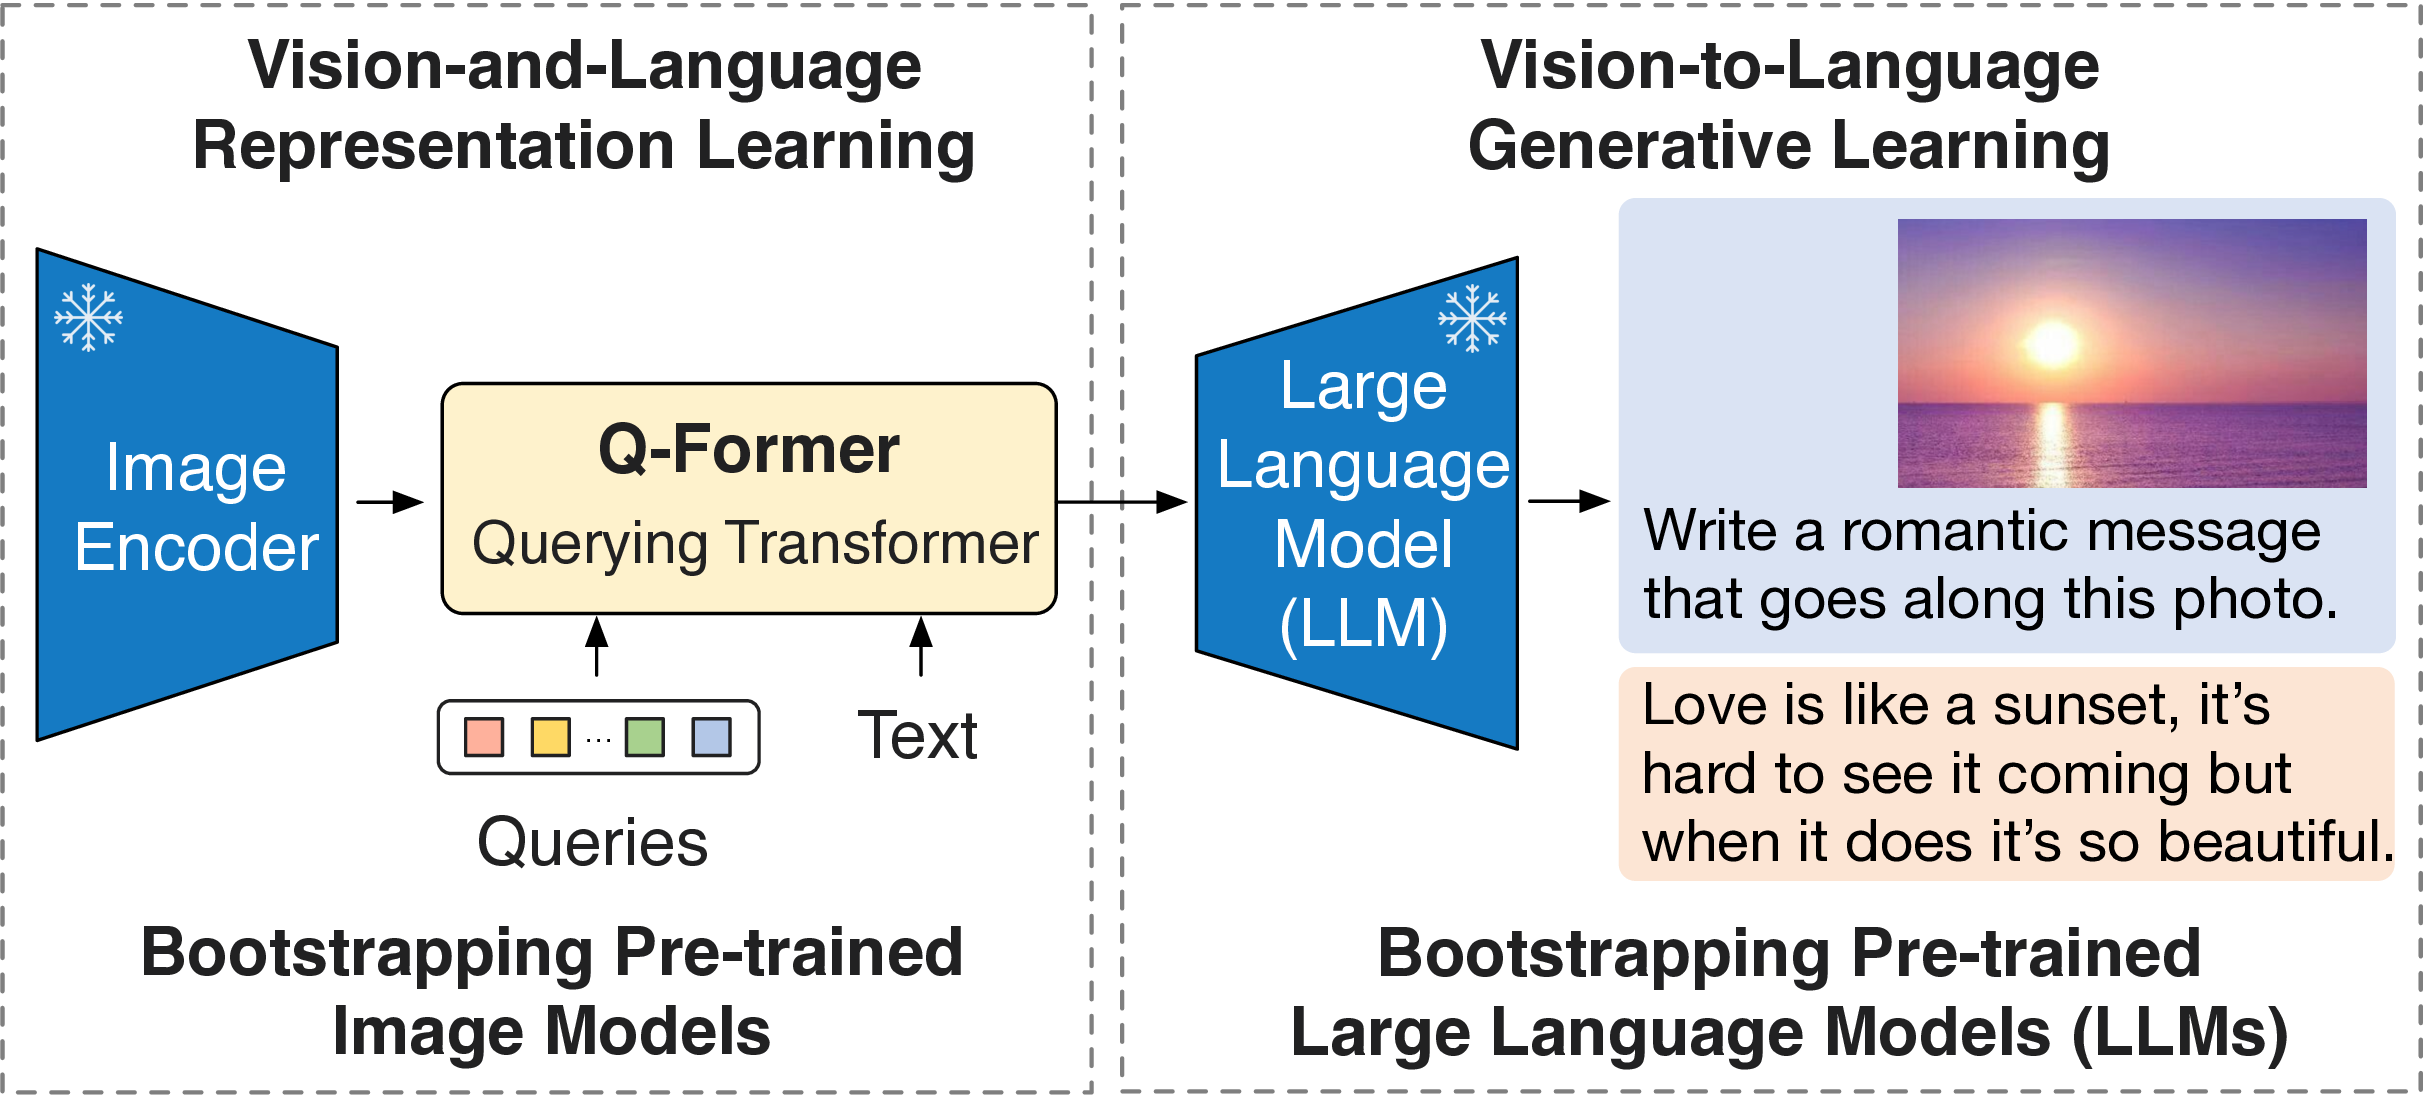
\includegraphics[width=0.8\textwidth]{assets/blip-2_arch.png}
  \caption{BLIP-2 网络结构} 
  \label{fig:blip2_structure} 
\end{figure}

    \begin{itemize}
\tightlist
\item
  LLaVA
  网络结构\cite{liu2023visualinstructiontuning}：直接用一个线性投影层\(W\)将视觉编码器的输出映射到语言模型的词嵌入空间。
\end{itemize}

\begin{figure}[h!]  % [h!]：优先将图片放在当前位置（here），避免乱跑
  \centering  % 图片居中显示
  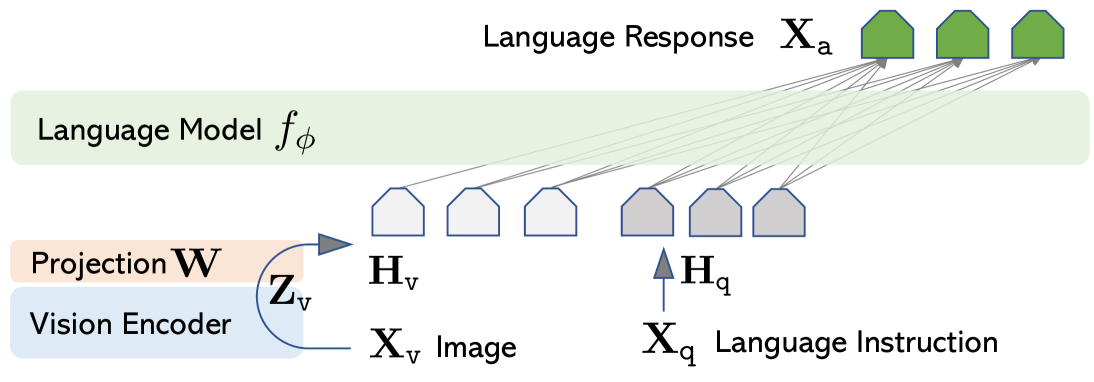
\includegraphics[width=0.8\textwidth]{assets/llava_arch1.png}
  \caption{LLaVA 网络结构} 
  \label{fig:llava_structure} 
\end{figure}

  \begin{itemize}
\tightlist
\item
  MiniGPT-4 网络结构\cite{zhu2023minigpt4enhancingvisionlanguageunderstanding}：采用冻结的BLIP-2预训练组件(EVA-CLIP中的ViT-g/14 和
  Q-Former)作为视觉编码器，通过线性投影层将Q-Former输出的视觉特征映射到LLM的输入空间。
\end{itemize}

\begin{figure}[h!]  % [h!]：优先将图片放在当前位置（here），避免乱跑
  \centering  % 图片居中显示
  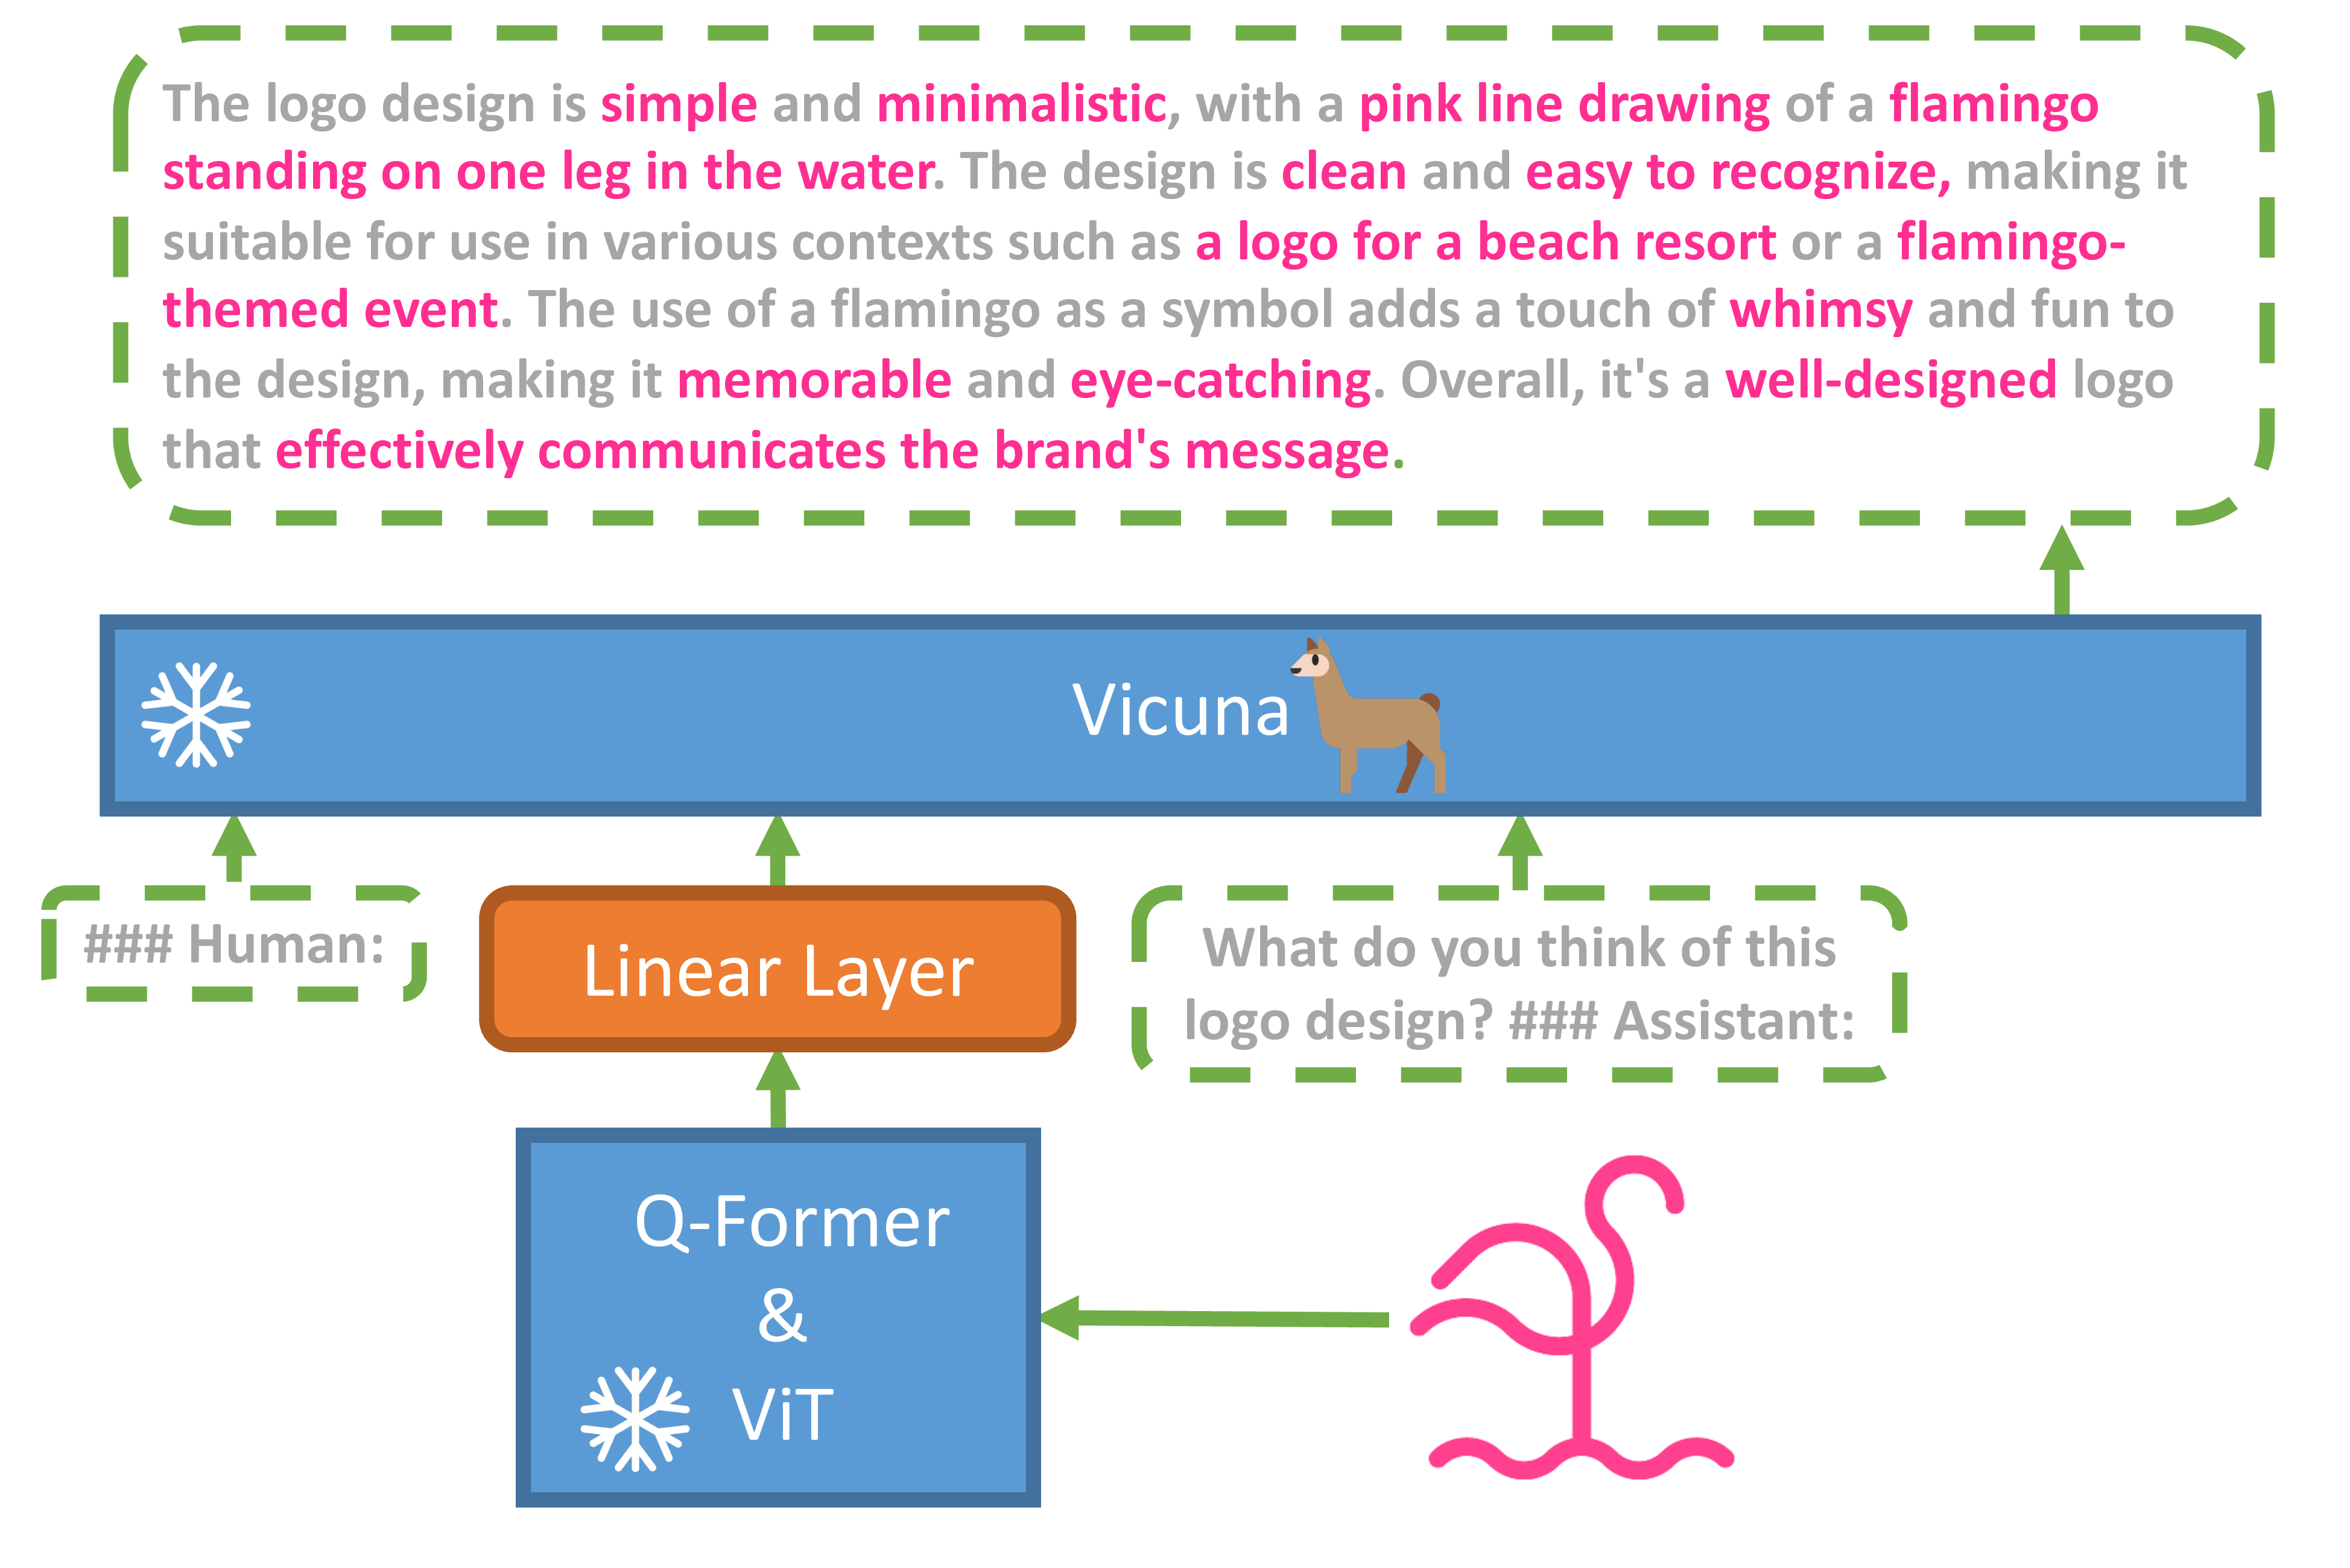
\includegraphics[width=0.8\textwidth]{assets/minigpt4_arch.png}
  \caption{MiniGPT-4 网络结构} 
  \label{fig:minigpt4_structure} 
\end{figure}

\subsection{网络结构背后的深度分析}
\textbf{LLaVA和MiniGPT-4选择Vicuna的核心原因:}
\begin{itemize}
\tightlist
\item
Vicuna对话与指令能力接近主流的闭源模型。Vicuna基于LLaMA构建，通过大量高质量的对话数据微调，在人类评估中对话性能达到ChatGPT的90\%\cite{vicuna2023}。多模态的核心需求之一是理解用户自然语言指令并生成连贯回复。比如根据图像生成食谱，解释图像中的异常现象等。Vicuna提供强大的逻辑和语言生成能力，以及零样本学习能力，远超当时BLIP-2所用的Flan-T5、OPT等模型。相比之下，同期其他模型则稍逊一筹。
\item
Vicuna的模型参数规模(7B/13B)适中，虽然LLaVA和MiniGPT-4在预训练阶段都冻结了Vicuna的参数。但是适中的模型参数规模让后续的微调成为可能，例如LLaVA二阶段中就解冻了Vicuna模型并在其构建的高质量指令数据集上微调。

\item
Vicuna完全开源且基于LLaMA的代码框架简洁易懂。团队可以快速使用并验证其性能。开源的特性让开发者能灵活调整模型的输入输出格式，更便捷地调整多模态的输入输出接口。

\item
且Vicuna团队后续整理出来"LLM-as-a-judge"方法\cite{zheng2023judgingllmasajudgemtbenchchatbot}，即用GPT-4等LLM作为语言生成内容的评估助手，这个想法也在LLaVA和MiniGPT-4中被使用。

\end{itemize}

\textbf{注意力还是简单的线性层:}
\begin{itemize}
\tightlist
\item
BLIP-2模型架构中，作者使用Q-Former作为跨模态连接的桥梁，Q-Former通过自注意力机制和跨注意力机制来融合和提取图像和文本的联合表示。这种设计允许模型更好地捕捉图像和文本之间的复杂关系，从而提升多模态任务的性能。但结构也相对复杂，计算资源消耗较大。
\item
LLaVA中选择了更简单的线性投影层来直接将视觉特征映射到语言模型的输入空间。线性层计算效率高，易于实现，且在实际应用中表现出色。但由于线性层没法捕捉图像编码器输出的块(patch)与块之间的关系，无法充分利用图像块间的空间信息。而Q-Former通过注意力机制能够更好地建模这些关系。
\item
在MiniGPT-4中，作者尝试了移除和保留Q-Former结构。实验证明，移除和保留Q-Former结构在AOK-VQA和GQA数据集上的表现差异不大，说明在某些任务中，简单的线性映射已经足够有效，复杂的注意力机制未必带来显著提升。
\end{itemize}


\subsection{训练策略}\label{ux8badux7ec3ux7b56ux7565}

\textbf{BLIP-2:}

% \begin{itemize}
% \tightlist
% \item
  阶段一：视觉-语言特征对齐预训练（冻结视觉编码器，仅训练Q-Former）

  \begin{itemize}
  \tightlist
  \item
    数据集：和BLIP相同（COCO, Visual Genome, CC3M, CC12M,SBU, 115M from
    LAION-400M）；使用CapFilt方法来创建人工注解。
  \item
    损失函数：使用大规模图像-文本对，通过聚合图像-文本对比损失(ITC)、图像-文本匹配损失(ITM)和图像-文本生成损失(ITG)三种损失来优化模型
  \item
    目标：使视觉特征与语言特征在语义空间中对齐，输出和文本最相关的视觉特征表示。
    \begin{figure}[h!]  % [h!]：优先将图片放在当前位置（here），避免乱跑
      \centering  % 图片居中显示
      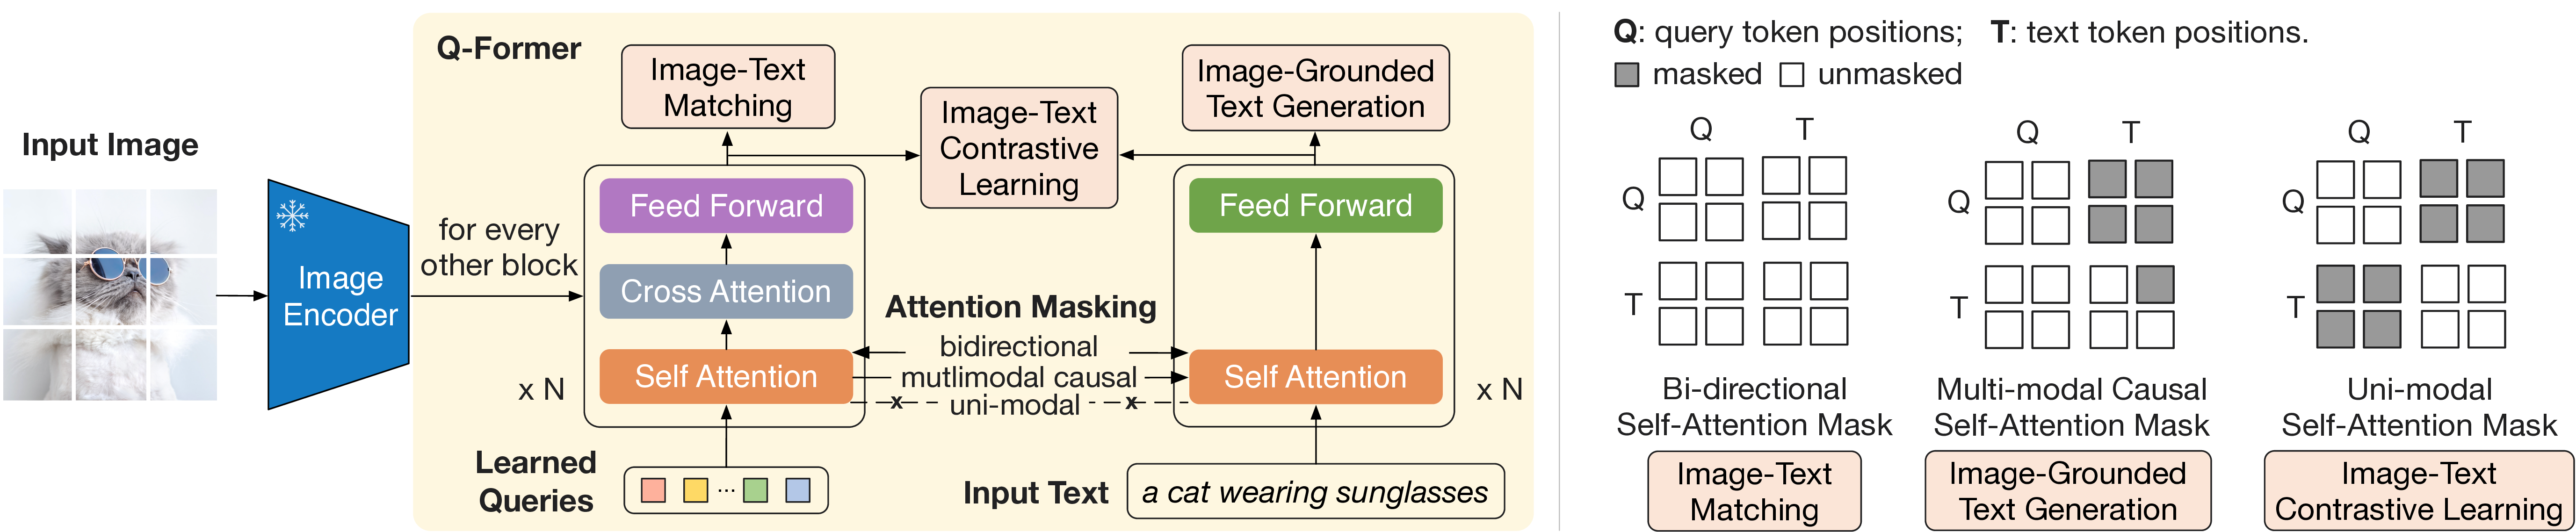
\includegraphics[width=0.8\textwidth]{assets/blip-2_stage1.png}
      \caption{BLIP-2 一阶段结构} 
      \label{fig:blip2_stage1}
    \end{figure}
  \end{itemize}
% \item
  阶段二：视觉-语言生成预训练（冻结视觉编码器和LLM，仅训练Q-Former和线性投影层）

  \begin{itemize}
  \tightlist
  \item
    损失函数：使用图像-文本对，通过文本生成交叉熵损失来优化模型
  \item
    目标：使其能够生成与图像内容相关的自然语言描述。

    \begin{figure}[h!]  % [h!]：优先将图片放在当前位置（here），避免乱跑
      \centering  % 图片居中显示
      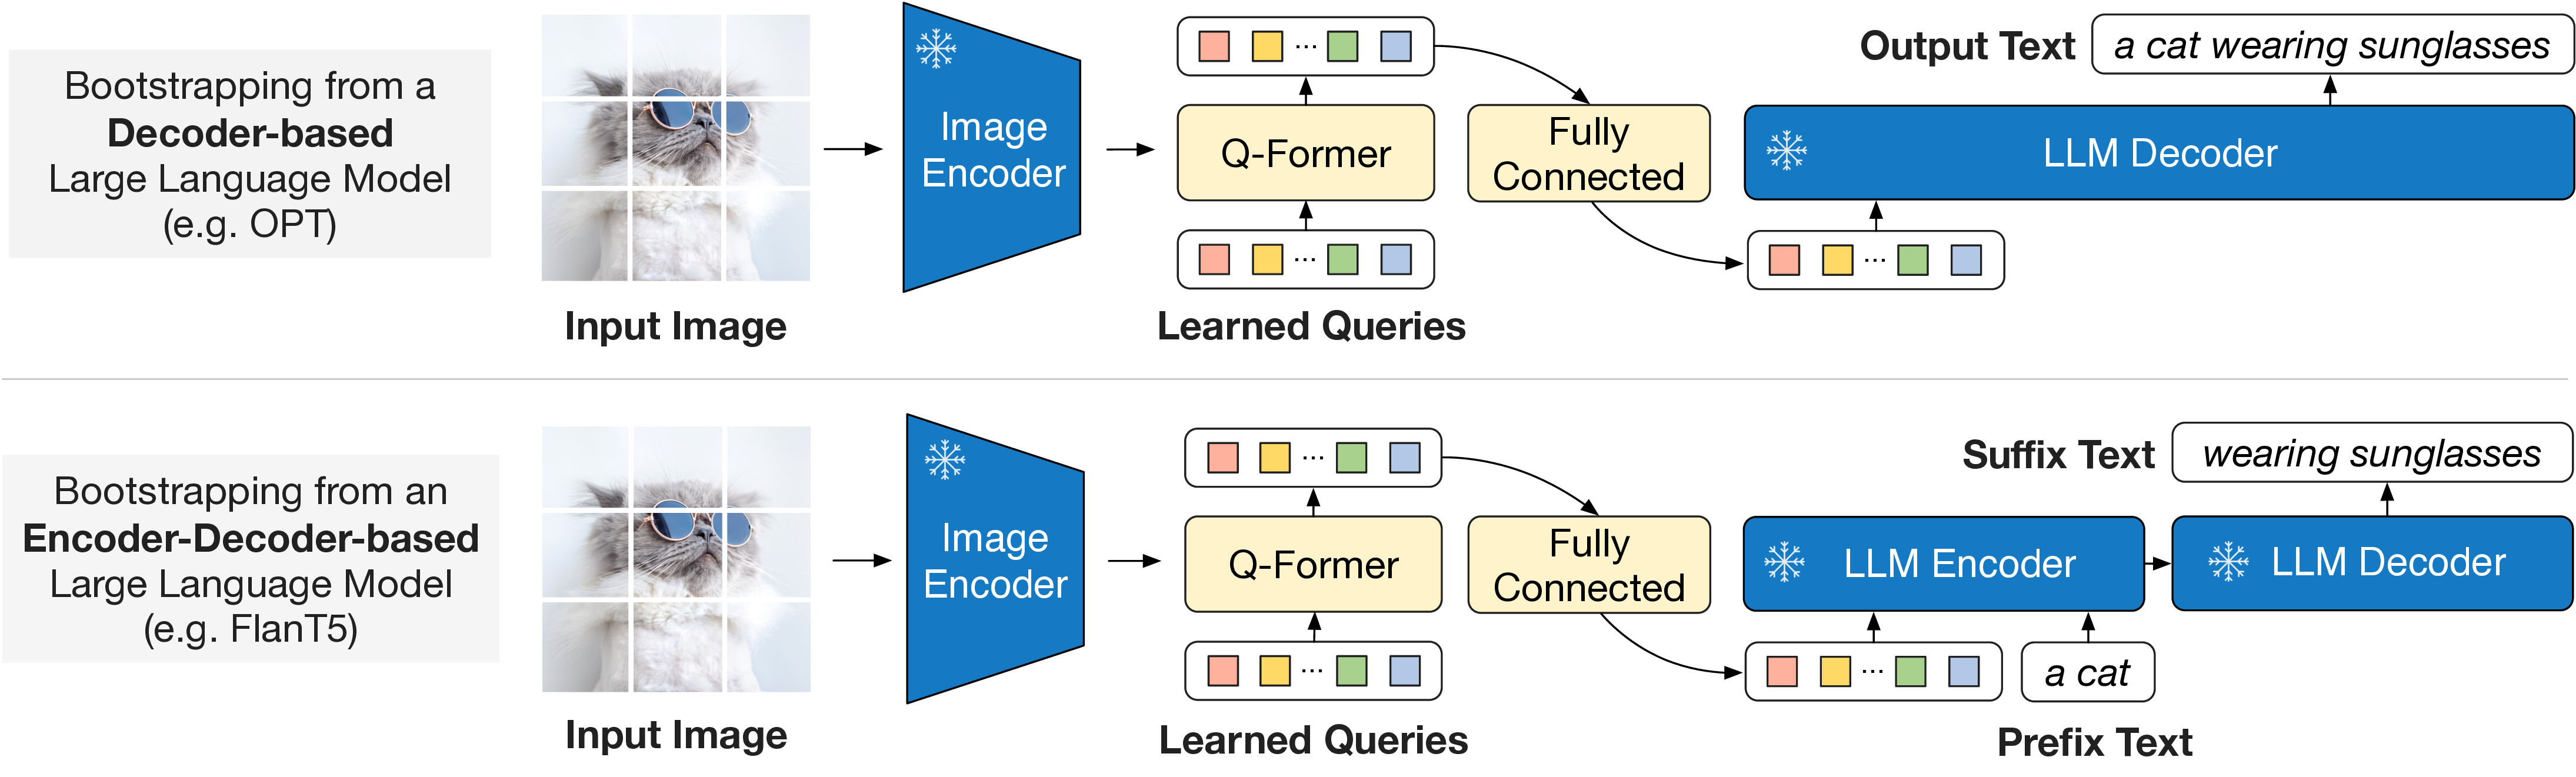
\includegraphics[width=0.8\textwidth]{assets/blip-2_stage2.png}
      \caption{BLIP-2 二阶段结构} 
      \label{fig:blip2_stage2}
    \end{figure}
  \end{itemize}
% \end{itemize}

\textbf{LLaVA:}

% \begin{itemize}
% \tightlist
% \item
  阶段一: 特征对齐的预训练 (更新\(W\))

  \begin{itemize}
  \tightlist
  \item
    数据集：使用CC3M筛选的595K图像-文本对
  \item
    损失函数：caption文本生成交叉熵损失
  \item
    目标：将视觉特征与语言模型的词嵌入空间对齐，使得视觉信息能够被语言模型有效利用
  \end{itemize}
% \item
  阶段二: 端到端微调 (更新\(W\)和语言模型参数)

  \begin{itemize}
  \tightlist
  \item
    数据集：利用GPT-4生成的158K视觉-语言指令跟随数据
  \item
    损失函数：多轮对话只关注\texttt{\textless{}STOP\textgreater{}}和生成回答的部分内容计算交叉熵损失
  \item
    目标：提升模型在复杂多模态任务中的理解和生成能力
  \end{itemize}
% \end{itemize}

    \textbf{MiniGPT-4:}

% \begin{itemize}
% \tightlist
% \item
  阶段一: 特征对齐预训练 (更新线性投影层)

  \begin{itemize}
  \tightlist
  \item
    数据集：Conceptual Caption, SBU和LAION数据集中的5M弱标注图像-文本对
  \item
    损失函数：文本生成损失
  \item
    出现的问题：生成不连贯的语言输出，如重复的词语、句子或无关内容（从GPT3.5受到启发，决定使用指令微调来解决这些问题）
  \end{itemize}
% \item
  阶段二: 指令微调 (更新线性投影层)

  \begin{itemize}
  \tightlist
  \item
    数据集：使用一阶段模型生成的3.5K高质量多模态指令数据(通过GPT-4辅助)；Localized
    Narratives数据集
  \item
    损失函数：指令跟随生成损失（不包含指令部分）
  \item
    目标：优化一阶段出现的问题，使模型产生更自然、可靠的语言输出
  \end{itemize}
% \end{itemize}

\section{定量分析}

本节所有数据均从LVLM-eHub\cite{xu2023lvlmehubcomprehensiveevaluationbenchmark}中获取。所有用于评估的模型相关参数可以在表\ref{tab:comparison-LVLMs}中找到。

\begin{figure}[h!]  % [h!]：优先将图片放在当前位置（here），避免乱跑
  \centering  % 图片居中显示
  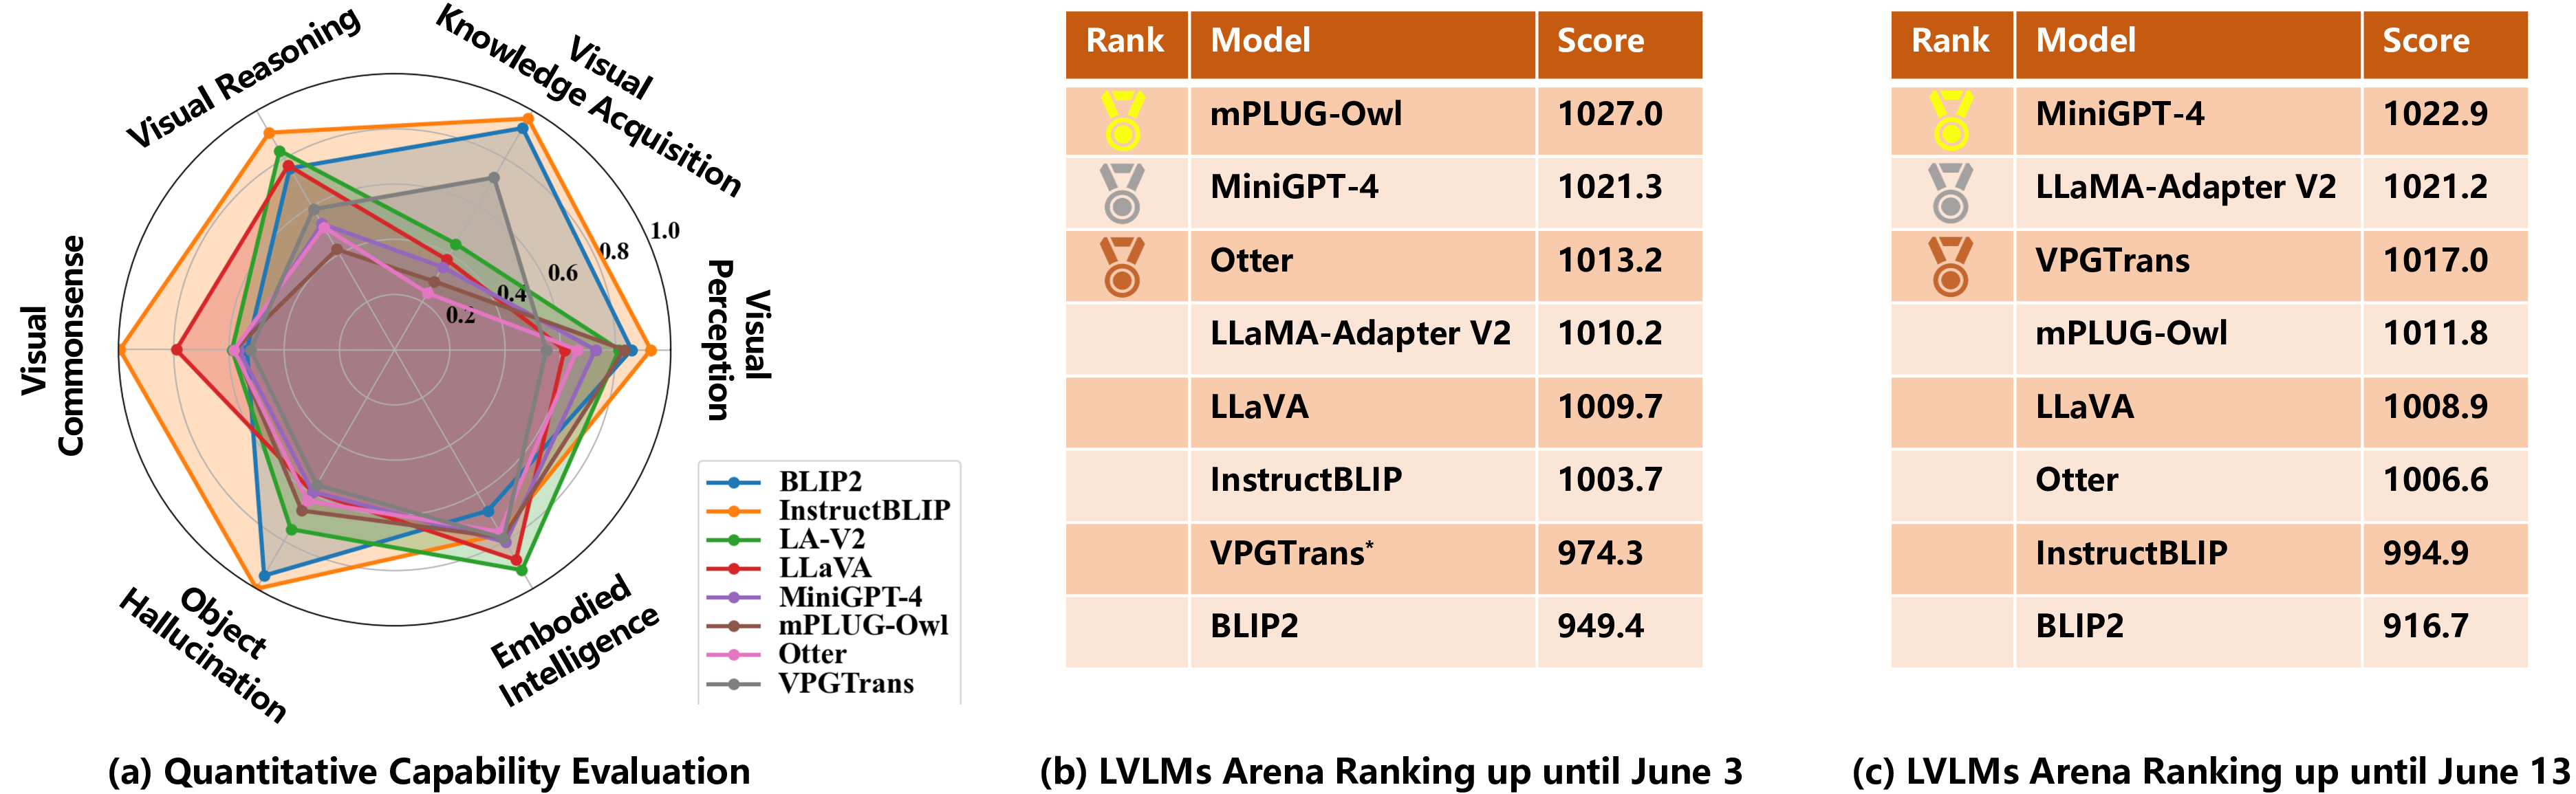
\includegraphics[width=0.8\textwidth]{assets/lvlm_ranking.png}
  \caption{LVLM 排名情况（2023年6月）} 
  \label{fig:lvlm_ranking}
\end{figure}

\begin{table*}[t]
\centering
\small
\resizebox{\textwidth}{!}{%
\begin{tabular}{c|cccccc|cc|cc}
\toprule
\multirow{2}{*}{Model} & \multicolumn{6}{c|}{Model Configuration} & \multicolumn{2}{c|}{Image-Text Data} & \multicolumn{2}{c}{Visual Instruction Data}  \\
\cmidrule{2-11}
& VE      & LLM    & Adapt &ToP &TuP &\# Token      & Source  & Size     & Source                  & Size      \\
\cmidrule{1-11}
BLIP2 & ViT-g/14$^\dag$      & FlanT5-XL$^\dag$   & Q-Former &4B &107M & 32      & CC$^*$-VG-SBU-L400  & 129M     & -                  & - \\
LLaVA & ViT-L/14$^\dag$     & Vicuna   & FC layer &7B &7B & 256     & CC3M  & 595K     & LLaVA-I                  & 158K \\
LA-V2 & ViT-L/14$^\dag$      & LLaMA$^\dag$   & B-Tuning &7B &63.1M &10      & L400  & 200M     & LLaVA-I                 & 158K \\
MiniGPT-4 & BLIP2-VE$^\dag$   & Vicuna$^\dag$   & FC layer &7B & 3.1M & 32      & CC-SBU-L400  & 5M     & CC+ChatGPT                 & 3.5K \\
InstructBLIP &ViT-g/14$^\dag$ & Vicuna$^\dag$ & Q-Former &7B & 107M & 32      & -  & -    & QA$^*$                & 16M \\ 
\bottomrule
\end{tabular}%
}
\caption {\textbf {不同多模态大语言模型（LVLM）对比表}。VE、Adapt、ToP、TuP 和 \# Token 分别表示视觉编码器（Visual Encoder）、适配模块（Adaption Module）、总参数量（Number of Total Parameters）、微调参数量（Tuning Parameters）以及输入到大语言模型（LLM）的视觉令牌数（Visual Tokens）。
%More visual tokens usually indicate better modeling of the global context in the image. 
$^\dag$ 表示该模型组件处于冻结状态（Frozen）。CC$^*$ 数据集包含(COCO , CC3M 和 CC12M).  CC, VG, CY, L400, LC 分别表示 Conceptual Caption , Visual Genome~, COYO-700M , LAION 400M~ 和 LAION COCO~ 数据集. SBU  包含 100万张带注解的图片. LLaVA-I 表示 在LLaVA中使用的158K多模态指令-跟随数据集. QA$^*$表示 InstructBLIP 模型所用的 13 个问答数据集。}
\label{tab:comparison-LVLMs}
\end{table*}

\subsection{视觉感知能力}

\begin{table*}[h!]
\centering
\small
\resizebox{\textwidth}{!}{%
\begin{tabular}{c|c|cccccc}
\toprule
\multicolumn{2}{c|}{Datasets} & BLIP2 & InstructBLIP & LA-V2 & LLaVA & MiniGPT-4 & S-SOTA \\
\cmidrule(lr){1-2}\cmidrule(lr){3-8}
\multirow{3}{*}{ImgCls}
& ImageNet1K & 23.71 & \underline{24.51} & \textbf{25.89} & 23.50 & 21.17 & 91.10~\\ 
& CIFAR10 & 58.20 & \underline{67.24} & 64.86 & \textbf{67.96} & 61.39 & 99.70~ \\ 
& Pets37 & \underline{34.79} & \textbf{38.86} & 24.39 & 9.09 & 18.90 &  96.70~ \\ 
& Flowers102 & 19.44 & \underline{21.78} & \textbf{22.34} & 8.38 & 21.70 & 99.64~ \\
\cmidrule(lr){1-2}\cmidrule(lr){3-8}
\multirow{2}{*}{OC}
& COCO  & \textbf{48.90} & \underline{46.65} & 38.50 & 20.56 & 20.86 & - \\
& VCR  & 25.05 & \textbf{29.29} & \underline{26.51} & 24.60 & 25.26 & -\\
\cmidrule(lr){1-2}\cmidrule(lr){3-8}
\multirow{2}{*}{MCI}
& COCO  & \underline{86.06} & \textbf{87.81} & 82.90 & 49.66 & 72.70 & - \\
& VCR   & 66.59 & \textbf
{76.49} & 50.66 & \underline{66.90} & 66.02 & - \\
\cmidrule(lr){1-2}\cmidrule(lr){3-8}
\multicolumn{2}{c|}{Average Score}
% & \underline{0.859} & \textbf{0.946} & 0.817 & 0.613 & 0.744 & 0.597 & 0.665 & 0.510  & - \\
& \underline{0.858} & \textbf{0.928} & 0.813 & 0.615 & 0.727 & - \\
\bottomrule
\end{tabular}%
}
\caption{多模态大语言模型（LVLMs）在图像分类（Imgcls）、目标计数（OC）和多类别识别（MCI）任务上的视觉感知能力评估结果。所有任务均采用准确率（accuracy）作为评估指标。其中，\textbf {最优结果} 以 \textbf {粗体} 标注，\underline {次优结果} 以 \underline {下划线} 标注。平均得分为每行数据归一化后取列均值计算得出。S-SOTA 代表有监督最优性能（supervised state-of-the-art）结果。}
% \leim{row `Avg.' updated based on (x / row\_max(x)) .avg\_column, note 8 rows in total}}
\label{tab:oc_mci_results}
\end{table*}

从表\ref{tab:oc_mci_results}可以看出，在大部分图像分类等任务中。各模型之间的表现较为接近。但是可以观察到（1）在Pets37和Flowers102数据集上，LLaVA的表现明显低于其他模型。这可能是因为简单的线性映射无法充分捕捉细粒度的图像特征以及利用图像块间的空间信息，从而影响了模型在细粒度分类任务中的表现。LLaVA 1.5\cite{liu2024improvedbaselinesvisualinstruction}中通过引入更复杂的MLP结构，性能上有所提升。（2）InstructBLIP在几乎所有任务上表现都优于其他模型，这可能是因为他在160万视觉问答(VQA)数据集上微调，使其在这类任务上过拟合。


\subsection{视觉知识获取能力}

\begin{table*}[h!]
\centering
\small
\resizebox{\textwidth}{!}{%
\begin{tabular}{c|c|cccccc}
\toprule
\multicolumn{2}{c|}{Datasets} & BLIP2 & InstructBLIP & LA-V2 & LLaVA & MiniGPT-4 & S-SOTA \\
\cmidrule(lr){1-2}\cmidrule(lr){3-8}
\multirow{13}{*}{OCR}
& IIIT5K      & \underline{80.17} & \textbf{83.90} & 36.30 & 31.57 & 25.00 & 99.2 \\
& IC13        & \underline{81.13} & \textbf{82.08} & 20.87 & 16.39 & 16.69 & 98.4 \\
& IC15        & \underline{66.68} & \textbf{73.57} & 29.40 & 26.58 & 22.05 & 91.4 \\
& Total-Text  & \underline{68.31} & \textbf{71.51} & 30.93 & 24.51 & 18.65 & 90.5 \\
& CUTE80      & \underline{85.07} & \textbf{86.11} & 35.76 & 36.46 & 33.33 & 99.3 \\
& SVT         & \underline{85.78} & \textbf{86.86} & 20.40 & 18.55 & 15.46 & 98.3 \\
& SVTP        & \underline{77.34} & \textbf{80.93} & 31.01 & 27.44 & 20.31 & 97.2 \\
& COCO-Text   & \underline{53.62} & \textbf{58.25} & 20.94 & 18.05 & 11.86 & 81.1 \\
& WordArt     & \underline{73.66} & \textbf{75.12} & 38.98 & 35.87 & 31.90 & 72.5 \\
& CTW         & \underline{67.43} & \textbf{68.58} & 18.13 & 16.73 & 14.95 & 88.3 \\
& HOST        & \underline{57.28} & \textbf{61.22} & 16.60 & 15.94 & 13.45 & 77.5 \\
& WOST        & \underline{68.83} & \textbf{73.26} & 21.73 & 20.49 & 19.12 & 87.5 \\
\cmidrule(lr){1-2}\cmidrule(lr){3-8}
\multirow{2}{*}{KIE}
& SROIE & \underline{0.08} & \textbf{0.09} & 0.02 & 0.01 & 0.02 & 97.81 \\
& FUNSD & 1.02 & 1.03 & \textbf{2.16} & \underline{1.93} & 1.27 & 89.45 \\
\cmidrule(lr){1-2}\cmidrule(lr){3-8}
\multirow{3}{*}{Image Captioning}
& NoCaps     & \textbf{48.58} & \underline{46.33} & 41.66 & 33.09 & 42.43 & 124.77 \\
& Flickr-30k & \underline{46.48} & \textbf{50.45} & 30.49 & 27.65 & 26.04 & - \\
& WHOOPS & \underline{96.12} & \textbf{97.98} &  57.60 &  34.36 &  47.36 & - \\
\cmidrule(lr){1-2}\cmidrule(lr){3-8}
\multicolumn{2}{c|}{Average Score} & \underline{0.927} & \textbf{0.967} & 0.443 & 0.377 & 0.346 & - \\
\bottomrule
\end{tabular}}
\caption{大规模多模态大语言模型（LVLMs）在光学字符识别（OCR）、关键信息提取（KIE）和图像描述（Image Captioning）任务上的零样本性能对比。评估指标包括：OCR 数据集采用词准确率（word accuracy）、KIE 数据集采用实体级 F1 分数（entity-level F1 score）、图像描述数据集采用 CIDEr 分数。}
\label{tab:vka_results}
\end{table*}

从表\ref{tab:vka_results}可以看出，BLIP-2和InstructBLIP在所有任务上都展现明显的优势。这可能是因为它采用了大型视觉编码器(ViT-g/14)和更复杂的特征提取模块(Q-Former)。使其能够通过注意力机制融合全局以及局部的图像视觉特征。

\subsection{视觉推理能力}

\begin{table*}[h!]
\centering
\small
\resizebox{\textwidth}{!}{%
\begin{tabular}{c|c|cccccc}
\toprule
\multicolumn{2}{c|}{Datasets} & BLIP2 & InstructBLIP & LLaMA-Adapter-v2 & LLaVA & MiniGPT-4 & S-SOTA \\
\cmidrule(lr){1-2}\cmidrule(lr){3-8}
\multirow{10}{*}{VQA}
& DocVQA  &  4.75 &  5.89 & \textbf{ 8.13} & \underline{ 6.26} &  2.65 & 54.48 \\
& TextVQA & 31.98 & \underline{39.60} & \textbf{43.76} & 38.92 & 19.40 & 73.1 \\
& STVQA   & 20.98 & 28.30 & \textbf{32.33} & \underline{28.40} & 13.55 & - \\
& OCR-VQA & \underline{38.85} & \textbf{60.20} & 38.12 & 23.40 & 16.85 & - \\
& OKVQA   & 44.93 & \textbf{60.52} & \underline{55.93} & 54.36 & 37.48 & - \\
& GQA     & \underline{45.53} & \textbf{49.96} & 43.93 & 41.30 & 30.82 & 72.1 \\
& Visdial & 10.73 & \textbf{45.20} & 12.92 & \underline{14.66} & 10.31 & 68.92 \\
& IconQA  & \textbf{62.82} & \underline{56.25} & 41.83 & 42.95 & 37.59 & 83.62 \\
& VSR     & \textbf{63.63} & 41.28 & 50.63 & \underline{51.24} & 41.56 & 70.1 \\
& WHOOPS      & \underline{24.87} & \textbf{30.13} & 24.15 & 24.39 & 17.91 & - \\
\cmidrule(lr){1-2}\cmidrule(lr){3-8}
\multirow{2}{*}{KGID}
& ScienceQA IMG & \textbf{60.73} & 46.26 & \underline{54.19} & 49.33 & 25.43 & 92.53 \\
& VizWiz        & \textbf{65.44} & \underline{65.31} & 62.07 & 62.42 & 47.48 & 73.3 \\
\bottomrule
\cmidrule(lr){1-2}\cmidrule(lr){3-8}
VE & SNLI-VE & 32.00 & \textbf{59.00} & \underline{58.8} & 57.80 & 54.80 & - \\
\cmidrule(lr){1-2}\cmidrule(lr){3-8}
\multicolumn{2}{c|}{Average Score} & 0.759 & \textbf{0.908} & \underline{0.833} & 0.771 & 0.527 & - \\
\bottomrule
\end{tabular}%
}
\caption{多模态大语言模型（LVLM）在视觉问答（VQA）、知识图谱问答（KGID）和视觉推理（VE）任务上的零样本性能对比。对于视觉问答（VQA）和知识图谱问答（KGID）任务，视觉对话数据集（Visdial）采用平均倒数排名（MRR）作为评估指标，其余任务均采用 top-1 准确率。}
\label{tab:vr_results}
\end{table*}

从表\ref{tab:vr_results}可以看出，（1）InstrcutBLIP之外，其他通过指令微调的LVLM的整体表现较差。作者分析这可能是由于目前的指标无法衡量指令表述对生成内容的影响。（2）在需要多轮推理的SNLI-VE任务中。所有通过指令微调的LVLM均优于BLIP-2，这也证明了指令微调在提升模型推理能力方面的有效性。


\subsection{视觉常识推理能力}
\begin{table*}[h!]
\centering
\small

\resizebox{\textwidth}{!}{%
\begin{tabular}{c|c|cccccc}
\toprule
\multicolumn{2}{c|}{Datasets} & BLIP2 & InstructBLIP & LA-v2 & LLaVA & MiniGPT-4 & S-SOTA \\
\cmidrule(lr){1-2}\cmidrule(lr){3-8}
\multirow{6}{*}{ImageNetVC}
& Color  & 26.22 & \textbf{67.78} & 36.12 & \underline{43.70} & 24.49 & 44.70 \\
& Shape  & 34.21 & \textbf{59.06} & 28.63 & \underline{39.10} & 23.54 & 40.50 \\
& Mater. & 35.79 & \underline{63.50} & 33.86 & \textbf{65.58} & 28.56 & 61.90 \\
& Compo. & 50.71 & \textbf{83.25} & 50.13 & 56.73 & \underline{59.26} & 54.00 \\
& Others & 34.48 & \textbf{68.37} & 32.69 & \underline{59.38} & 39.38 & 51.70 \\
\cmidrule(lr){1-2}\cmidrule(lr){3-8}
%\multirow{2}{*}{Whoops}
%& Identify  &  &  &  &  &  &  &  &  & \\
%& Explain   &  &  &  &  &  &  &  &  & \\
\cmidrule(lr){1-2}\cmidrule(lr){3-8}
VCR & VCR & 31.60 & \textbf{54.20} & \underline{49.80} & 48.20 & 49.00 & - \\
\cmidrule(lr){1-2}\cmidrule(lr){3-8}
\multicolumn{2}{c|}{ Average Score} & 0.535 & \textbf{0.995} & 0.589 & \underline{0.791} & 0.565 & - \\
\bottomrule
\end{tabular}%
}
\caption {多模态大语言模型（LVLM）在 VCR 和 ImageNetVC 数据集上的零样本视觉常识推理性能对比。两个数据集均采用 top-1 准确率作为评估指标。}
\label{tab:vc_results}
\end{table*}

从表\ref{tab:vc_results}可以看出。（1）LLaVA在常识任务中表现优于BLIP2。这表明，相较于 BLIP2，指令微调能够为视觉常识任务提供更有效的线索。（2）在VCR（需要多轮推理）任务中，LLaVA和MiniGPT-4均优于BLIP-2，进一步验证了指令微调对于推理能力的提升。


\subsection{对象识别幻觉}
\begin{table*}[h!]
\centering
\small
\resizebox{\textwidth}{!}{%
\begin{tabular}{c|c|ccccc}
\toprule
Datasets & Metrics & BLIP2 & InstructBLIP & LA-V2 & LLaVA & MiniGPT-4 \\
\cmidrule(lr){1-2}\cmidrule(lr){3-7}
\multirow{5}{*}{MSCOCO-Random}
& Accuracy  & \underline{82.21} & \textbf{88.83} & 74.44 & 51.52 & 52.58 \\
& Precision & 97.48 & 96.01 & 68.24 & 51.54 & 68.63 \\
& Recall    & 67.27 & 81.60 & 94.00 & 100.00 & 57.50 \\
& F1-Score  & \underline{79.61} & \textbf{88.23} & 79.08 & 68.03 & 62.57 \\
& Yes       & 35.58 & 43.99 & 70.99 & 100.00 & 44.25 \\
%\bottomrule
\cmidrule(lr){1-2}\cmidrule(lr){3-7}
\multirow{5}{*}{MSCOCO-Popular}
& Accuracy  & \underline{80.10} & \textbf{84.15} & 56.82 & 50.00 & 49.31 \\
& Precision & 90.49 & 85.96 & 53.89 & 50.00 & 63.56 \\
& Recall    & 67.27 & 81.60 & 94.20 & 100.00 & 58.03 \\
& F1-Score  & \underline{77.17} & \textbf{83.72} & 68.56 & 66.67 & 60.67 \\
& Yes       & 37.17 & 47.47 & 87.40 & 100.00 & 48.29 \\
% \bottomrule
\cmidrule(lr){1-2}\cmidrule(lr){3-7}
\multirow{5}{*}{MSCOCO-Adversarial}
& Accuracy  & \underline{78.52} & \textbf{81.95} & 60.52 & 50.00 & 49.62 \\
& Precision & 86.83 & 82.05 & 54.58 & 50.00 & 62.55 \\
& Recall    & 67.27 & 81.60 & 96.45 & 100.00 & 58.71 \\
& F1-Score  & \underline{75.81} & \textbf{81.82} & 69.12 & 66.67 & 68.47 \\
& Yes       & 38.73 & 49.77 & 88.23 & 100.00 & 48.54 \\
\cmidrule(lr){1-2}\cmidrule(lr){3-7}
\multicolumn{2}{c|}{ Average Score} & \underline{0.945} & \textbf{1.00} & 0.751 & 0.595 & 0.594 \\
\bottomrule
\end{tabular}%
}
\caption {基于 POPE 评估框架的多模态大语言模型（LVLM）在 MSCOCO 数据集上的零样本性能详细评估结果。其中，准确率（accuracy）表示预测结果的正确率；精确率（precision）表示预测为正样本的结果中真实正样本的比例；召回率（recall）表示所有真实正样本中被正确识别的比例；“yes” 表示模型输出 “是” 答案的概率。平均得分为基于准确率指标计算得出。}
\label{tab:pope_results}
\end{table*}

从表\ref{tab:pope_results}可以看出，InstructBLIP在幻觉任务中表现优异，BLIP-2次之，而LLaVA和MiniGPT-4的表现较差，核心原因是后者更倾向于回答“是”。这表明LVLM容易生成图像中不存在的物体描述。作者随后又论证：多轮推理流程能够有效缓解此类物体幻觉问题。



\newpage

\section{创新点与局限性分析}\label{ux4e09ux7ed3ux8bba}
\subsection{创新点}

\begin{enumerate}
\def\labelenumi{\arabic{enumi}.}
\item
  BLIP-2：BLIP-2的核心突破在于其: 1)引入\textbf{Q-Former}这一轻量的跨模态桥梁模块。在冻结预训练视觉编码器和大语言模型的前提下，BLIP-2通过训练Q-Former实现了高效的视觉-语言特征对齐与融合，显著降低了训练成本。 2)提出了二阶段训练范式，先是视觉-语言表示预训练，然后是融合图像信息的语言生成能力的训练，为后续跨模态模型提供了重要参考。
\item
  LLaVA：LLaVA的创新聚焦于``轻量链接模块''和``高质量的指令微调数据集''相结合。在模型层面，它采用简单高效的线性投影层(LLaVA 1.5使用两个线性层的MLP)作为视觉-语言特征对齐的桥梁，结构更简洁且易于与开源大语言模型(如Vicuna)适配，降低了技术落地门槛；在数据层面，LLaVA通过GPT-4构建了``视觉指令调优数据集(LLaVA-Instruct-150K)''，通过``图像-注解-指令''的三元组数据形式，将通用图像描述转化为符合人类交互习惯的指令任务，使模型能够精准理解并回复复杂指令，显著提升了多模态对话的自然度与准确性。同时在微调过程中，LLaVA同时训练了连接模块和部分LLM参数，进一步增强了模型的适应能力。
\item
  MiniGPT-4：MiniGPT-4和LLaVA类似。两者都注重第二阶段的指令微调并都利用GPT-4辅助生成了高质量的多模态指令数据。但MiniGPT-4使用了更多的数据在一阶段的预训练中完成视觉-语言特征对齐，例如一阶段结束后，模型已经可以用来生成图像的详细描述并使用GPT-4辅助修改、纠正错误，从而为二阶段微调提供更高质量的指令数据集。此外，MiniGPT-4也尝试了不同的连接模块，如线性投影层/不带Q-Former的版本等等。和LLaVA本质的不同是没有微调LLM本身，节约了计算资源。
\end{enumerate}

\subsection{各模型的主要局限性}

\begin{enumerate}
\def\labelenumi{\arabic{enumi}.}
\item
  BLIP-2：BLIP-2的性能高度依赖所对接的大语言模型能力，若搭配的LLM（如Flan-T5）指令理解能力较弱，其多模态对话的灵活性会显著下降；由于使用的是CapFilt生成的注解，数据集本身质量可能不高。同时，由于其训练数据以通用图像描述为主，缺乏针对性的指令调优数据，在处理``图像编辑建议''\,``场景逻辑分析''等复杂指令时，响应的精准度与逻辑性不足。此外，Q-Former模块的训练需要依赖大规模视觉-文本预训练数据，对数据质量与数量的要求较高，增加了技术复现难度。当然，也继承了LLM本身的可能存在冒犯性语言、社会偏见、隐私泄漏等问题。
\item
  LLaVA：LLaVA采用的单个线性投影层虽结构简洁，但融合能力相对有限，难以充分捕捉图像中的细粒度特征，在处理``包含多个相似物体的场景识别''\,``微小视觉细节描述''等任务时表现较弱；LLaVA 1.5中通过尝试更复杂的MLP结构，并使用更高分辨率的视觉编码器以及13B的Vicuna模型，得到了一定提升。但还存在一个根本问题:
  bag of patches，
  即视觉编码器输出的patch特征是无序的，线性层难以捕捉空间关系，导致对复杂场景的理解能力受限。此外，LLaVA在微调过程中同时更新连接模块和部分LLM参数，虽然提升了模型适应性，但也增加了训练复杂度和计算资源需求。
\item
  MiniGPT-4：MiniGPT-4的大规模数据筛选与一阶段特征对齐训练时，需要消耗大量的计算资源，尤其是在使用高分辨率视觉编码器时，训练周期与成本显著高于LLaVA；此外，MiniGPT-4的视觉感知有限，难以区分空间定位。(可以通过RefCOCO和Visual Genome数据集进行训练)；以及MiniGPT-4继承了LLM本身的幻觉问题，且通过实验发现更长的回复往往伴随更高的幻觉率。
  % （潜在优化方向：使用AI幻觉检测模块进行强化学习）
\end{enumerate}

\subsection{局限性的潜在解决方案}

\begin{figure}[h!]  % [h!]：优先将图片放在当前位置（here），避免乱跑
  \centering  % 图片居中显示
  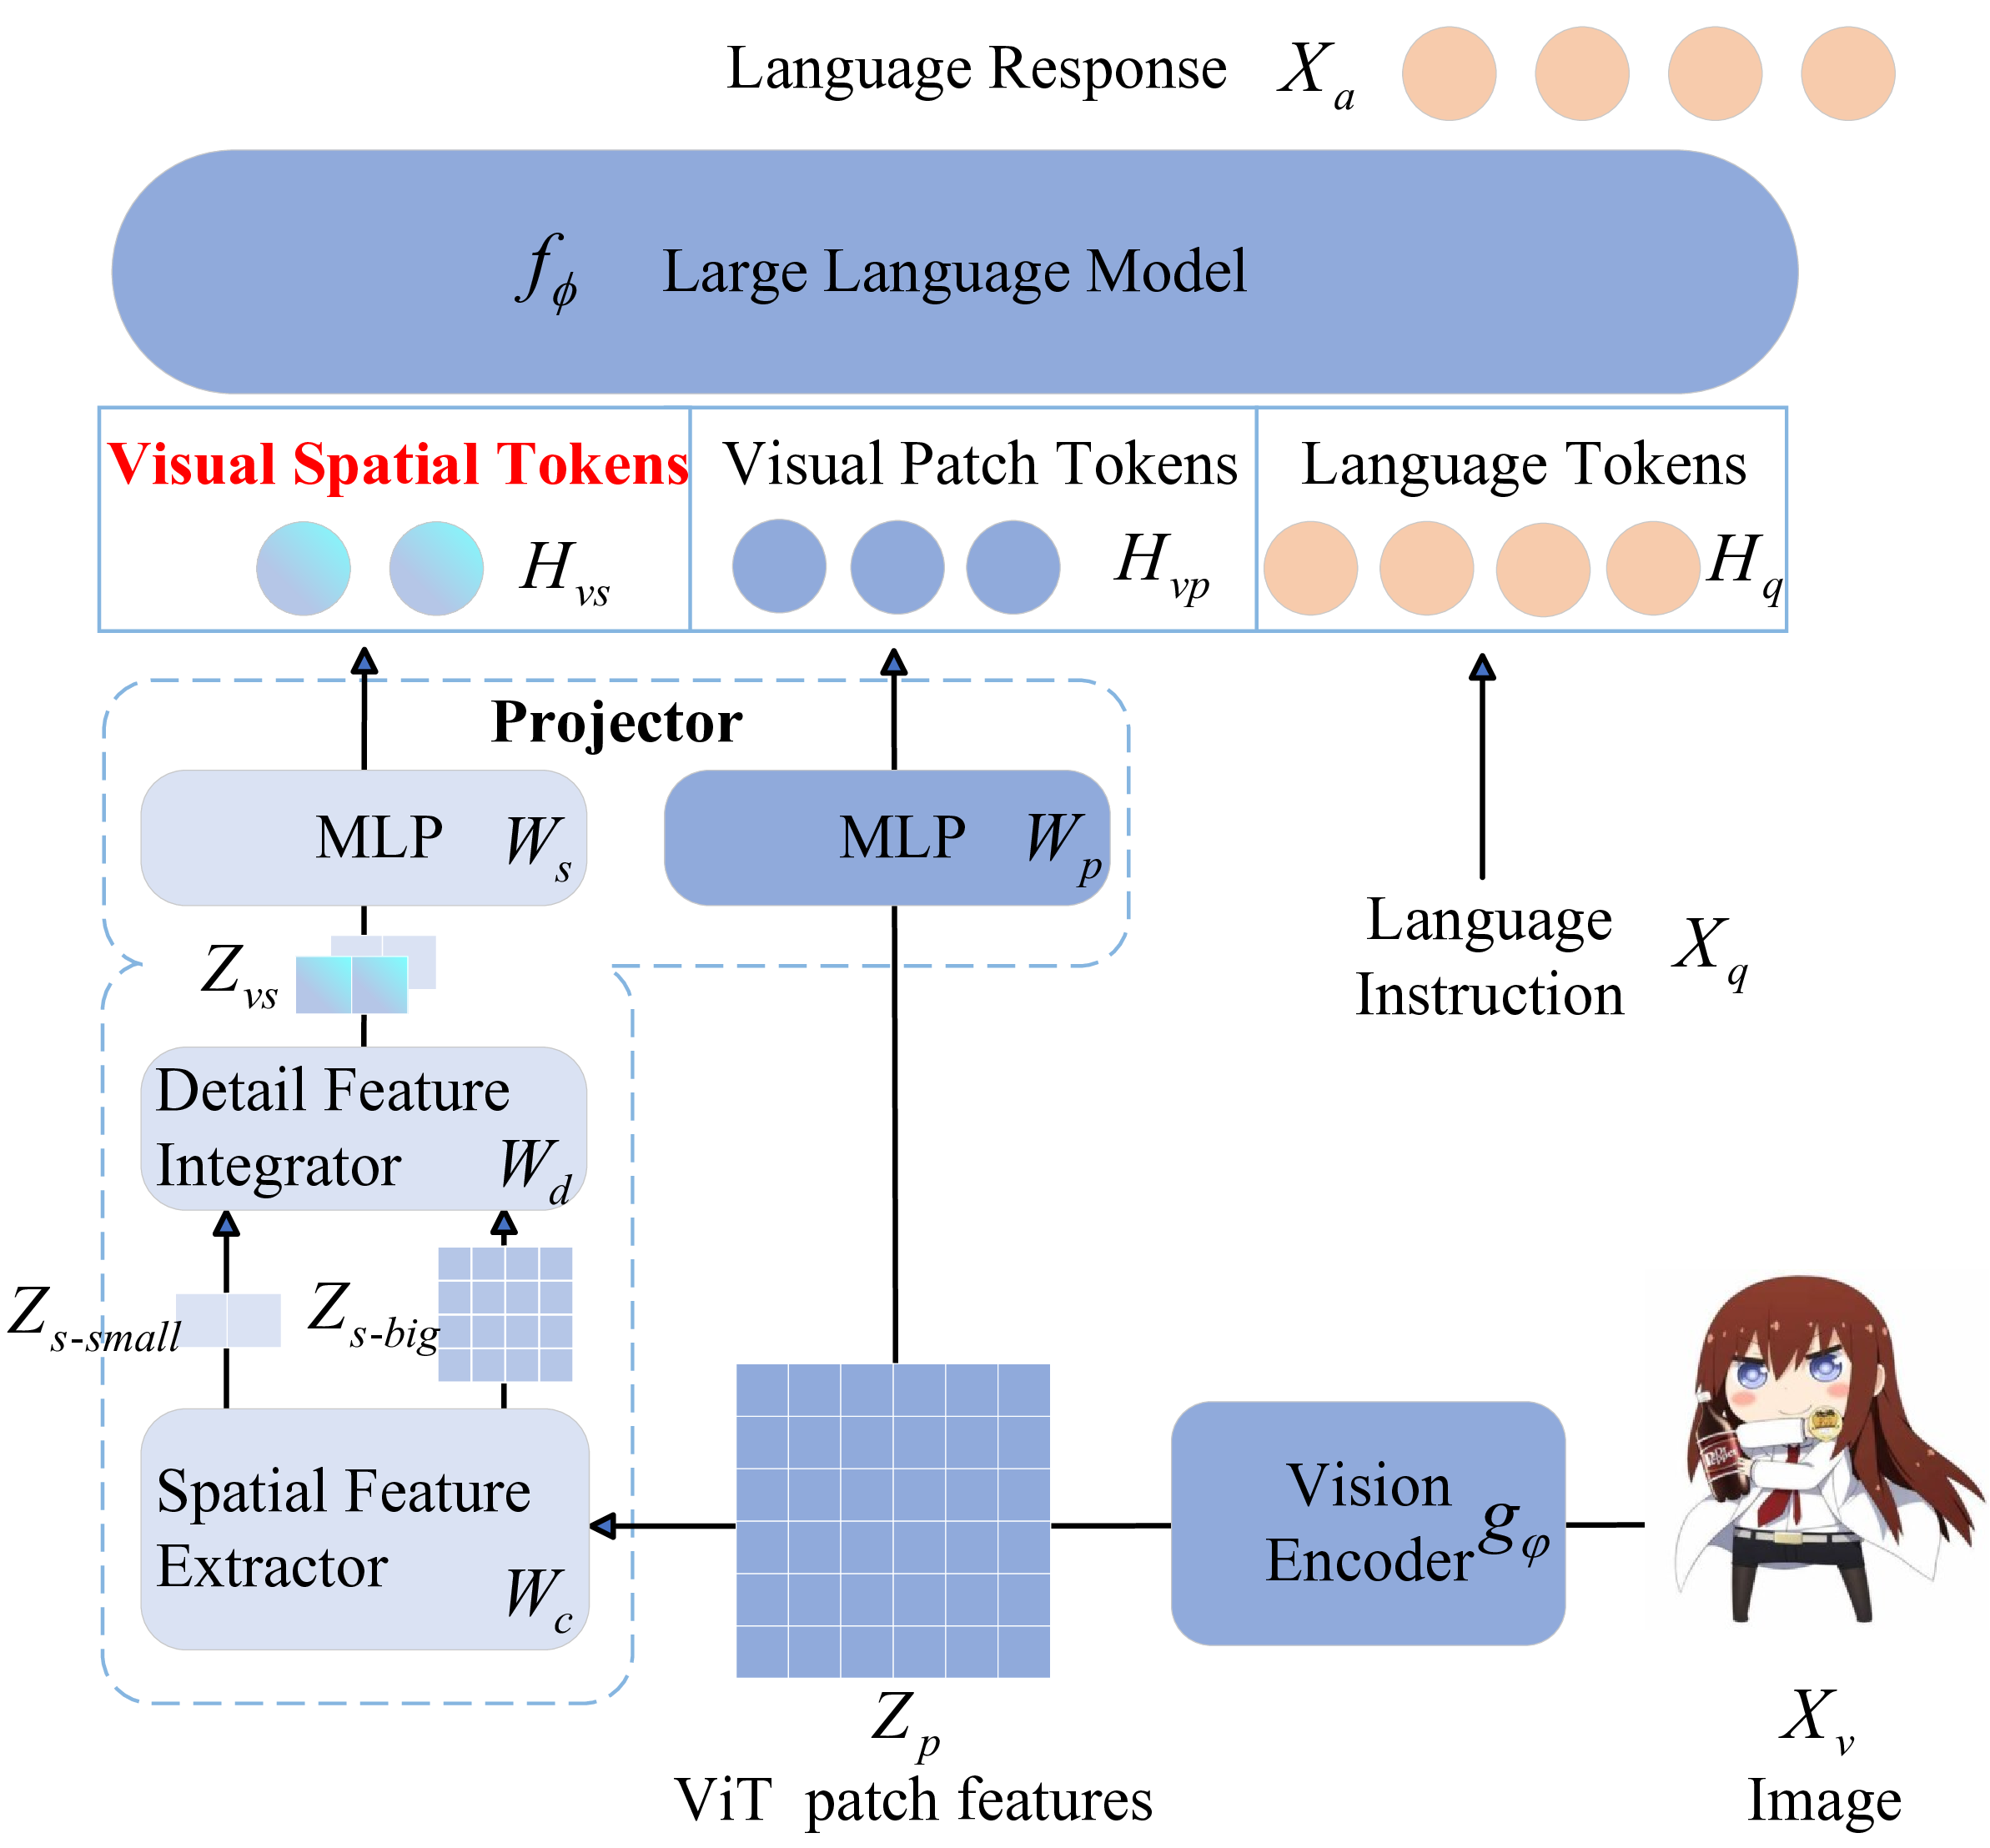
\includegraphics[width=0.8\textwidth]{assets/llava-sp_arch.png}
  \caption{LLaVA-SP 模型架构示意图}
  \label{fig:llava-sp_arch}
\end{figure}

\begin{table*}[t!]


%\scriptsize
\footnotesize
\centering
\setlength{\tabcolsep}{2pt}
\begin{tabular*}{1.0\linewidth}{l c c|c c c c c|c c c c c c}
\toprule
Method & LLM & Res. & VQA\textsuperscript{v2} & GQA & VizWiz & SQA\textsuperscript{I} & VQA\textsuperscript{T} & POPE & MME\textsuperscript{P} & MMB & SEED\textsuperscript{I} & LLaVA\textsuperscript{W} & MM-Vet\\
\midrule
BLIP-2~ & Vicuna-13B & 224 & 41.0 & 41.0 & 19.6 & 61.0 & 42.5 & 85.3 & 1293.8 & – & 46.4 & 38.1 & 22.4 \\

InstructBLIP~ & Vicuna-7B & 224 & – & 49.2 & 34.5 & 60.5 & 50.1 & – & – & 36.0 & 53.4 & 60.9 & 26.2    \\

InstructBLIP~ & Vicuna-13B & 224 & – &
49.5 & 33.4 & 63.1 & 50.7 & 78.9 & 1212.8 & – & – & 58.2 & 25.6 \\


Shikra~ & Vicuna-13B & 224 & 77.4 & – & – & – & – & – & – & 58.8 & – & – & –
\\

Qwen-VL~ & Qwen-7B & 448 & 78.8 & 59.3 & 35.2 & 67.1 & \textbf{63.8} & – & – & 38.2 & 56.3 & – & –    \\

Qwen-VL-Chat~ & Qwen-7B & 448 & 78.2 & 57.5 & 38.9 & 68.2 & \underline{61.5} & – & \underline{1487.5} & 60.6 & 58.2 & – & – \\

DeCo~ & Vicuna-7B & 336 & 74.0 & 54.1 & 49.7 & – & 56.2 & 85.9 & 1373.4 & 60.6 & 62.8 & – & – \\



LLaVA-1.5\dag~ & Vicuna-7B & 336 & 78.5 & 62.0 & 50.0 & 66.8 & 58.2 & 85.9 & \textbf{1510.7} & 64.3 & 66.2 & 63.4 & 30.5 \\
LLaVA-1.5*~ & Vicuna-7B & 336 & 78.4 & 61.9 & 45.7 & 67.6 & 56.2 & 85.8 & 1477.4 & 64.5 & 67.0 & 64.2 & 32.1 \\

\midrule
\rowcolor{gray!20}
LLaVA-SP-Cropping & Vicuna-7B & 336 & \underline{79.2} & \underline{62.4} & \underline{50.1} & \textbf{69.7} & 58.7 & \underline{86.4} & 1473.8 & \textbf{65.8} & \textbf{67.6} & \underline{66.7} & \underline{32.2} \\

\rowcolor{gray!20}
LLaVA-SP-Pooling & Vicuna-7B & 336 & 79.1 & \textbf{62.5} & \textbf{51.6} & \underline{69.0} & 58.3 & \textbf{86.5} & 1475.9 & \underline{65.7} & \underline{67.5} & \textbf{68.3} & \textbf{33.4} \\

\bottomrule
\end{tabular*}

\caption{\textbf {与现有最优（SoTA）方法在 11 个基准测试集上的性能对比}。两种基于 LoRA 微调的 LLaVA-SP 版本在 11 个基准测试集中的 10 个上超越了 LLaVA-1.5。}
\label{table:llava-sp-results}
\end{table*}


\subsubsection{针对bag of patches问题} 

在LLaVA-SP\cite{lou2025llavaspenhancingvisualrepresentation}中，作者通过引入空间特征提取器(Spatial Feature Extractor, SFE)模块，利用卷积神经网络(CNN)对视觉编码器输出的patch特征进行6个不同尺度的空间特征提取。并使用细节特征整合器(Detail Feature Integrator, DFI)模块，利用注意力机制将原始尺度的空间特征注入到6个不同尺度的特征中。最后再通过线性层添加到原始的视觉特征映射的前面。从表 \ref{table:llava-sp-results} 可以看出，LLaVA-SP在11个基准测试集中的10个上超越了LLaVA-1.5，验证了该方法的有效性。图\ref{fig:llava-sp_arch}展示了LLaVA-SP的整体架构示意图。


\begin{table*}[t]            
\centering          
\scalebox{0.68}{
\begin{tabular}{@{}llllllllll@{}}           
\toprule          
\multirow{2}{*}{\textbf{Decoding}} & \multirow{2}{*}{\textbf{Method}} &\multicolumn{2}{c}{\textbf{InstructBLIP}} &\multicolumn{2}{c}{\textbf{MiniGPT-4}} & \multicolumn{2}{c}{\textbf{LLaVA-1.5}} & \multicolumn{2}{c}{\textbf{Qwen-VL}}\\    
\cmidrule(lr){3-4} \cmidrule(lr){5-6} \cmidrule(lr){7-8} \cmidrule(lr){9-10}
  &  & $\mathrm{CHAIR_S}\downarrow$ & $\mathrm{CHAIR_I}\downarrow$ & $\mathrm{CHAIR_S}\downarrow$ & $\mathrm{CHAIR_I}\downarrow$ & $\mathrm{CHAIR_S}\downarrow$ & $\mathrm{CHAIR_I}\downarrow$ & $\mathrm{CHAIR_S}\downarrow$ & $\mathrm{CHAIR_I}\downarrow$ \\            
\midrule            
\multirow{2}{*}{\makecell[l]{Greedy}} & Vanilla & 58.8 & 23.7 & 31.8 & 9.9 & 45.0 & 14.7 & 46.0 & 12.5\\      
& DoLa & 48.4 & 15.9 & 32.2 & 10.0 & 47.8 & 13.8 & 46.8 & 12.9\\   
 & \textbf{DeCo} & \textbf{41.2\down{17.6}} & \textbf{14.4\down{9.3}} & \textbf{27.0\down{4.8}} & \textbf{8.8\down{1.1}} & \textbf{37.8\down{7.2}} & \textbf{11.1\down{3.6}} & \textbf{42.2\down{3.8}} & \textbf{10.7\down{1.8}} \\        
\cmidrule(l){1-10}      
\multirow{3}{*}{\makecell[l]{Beam Search}} & Vanilla & 55.6 & 15.8 & 30.6 & 9.5 & 48.8 & 13.9 & 41.8 & 10.8\\            
 & OPERA & 46.4 & 14.2 & 26.2 & 9.5 & 44.6 & 12.8 & 34.6 & 9.5\\           
 & \textbf{DeCo} & \textbf{43.8\down{11.8}} & \textbf{12.7\down{3.1}} & \textbf{24.8\down{5.8}} & \textbf{7.5\down{2.0}} & \textbf{33.0\down{15.8}} & \textbf{9.7\down{4.2}} & \textbf{32.0\down{9.8}} & \textbf{8.7\down{2.1}} \\          
\cmidrule(l){1-10}      
\multirow{3}{*}{\makecell[l]{Nucleus}} & Vanilla & 54.6 & 24.8 & 32.6 & 10.7 & 48.8 & 14.2 & 49.2 & 13.1\\            
 & VCD & 58.0 & 17.0 & 33.8 & 11.1 & 54.0 & 16.0 &  46.4 & 11.9\\           
 & \textbf{DeCo} & \textbf{43.6\down{11.0}} & \textbf{12.9\down{11.9}} & \textbf{30.8\down{1.8}} & \textbf{9.5\down{1.2}} & \textbf{42.8\down{6.0}} & \textbf{13.2\down{1.0}} & \textbf{43.8\down{5.4}} & \textbf{11.8\down{1.3}}\\         
\bottomrule          
\end{tabular}}
\caption{\textbf{CHAIR 幻觉评估结果}。
分数越低表示幻觉越少。
OPERA 采用束搜索（beam search），VCD 采用核采样（nucleus sampling），而 DeCo 是所提方法，可兼容多种解码策略。}
\label{tab:chair}            
\end{table*} 

\subsubsection{针对幻觉问题}
Deco\cite{wang2025mllmseedynamiccorrection} 论文中，作者分析了多模态大语言模型（MLLM）在视觉问答任务中产生幻觉的可能原因，发现可能源于语言模型的强知识先验抑制了视觉信息。为此，作者提出了一种动态纠正机制( Dynamic Correction Mechanism, DCM)，先在模型早期层中定位锚层(在a层到b层之间使得真实标记最大的层，实验中选择$a=20$ 和 $b = 28$)。再把锚层的视觉证据按动态权重融入最终层的逻辑值计算，以此平衡语言知识先验和视觉感知，避免视觉信息在解码中逐渐衰减。从表\ref{tab:chair}可以看出，DeCo在不同的解码策略下均显著降低了幻觉评分，验证了该方法的有效性。

\section{结论}

BLIP-2 创新性地引入 Q-Former 模块，通过跨模态注意力机制实现视觉与语言特征的深度匹配。该方案虽有效提升了视觉特征的细粒度表达能力，并部分保留了图像的空间结构信息，但其依赖预训练视觉编码器与 Q-Former 的两阶段训练范式，导致整体训练成本显著增加。相比之下，LLaVA 与 MiniGPT-4 从另一个维度验证了指令微调（Instruction Tuning）在多模态大语言模型（MLLM）中的核心价值 —— 通过构建高质量、多样化的指令遵循数据集，模型能够精准理解复杂任务意图，并高效支撑多轮对话与逻辑推理类任务的响应需求。
LLaVA 最初采用的单一线性层方案，为视觉 - 语言特征对齐提供了轻量、低成本的实现路径，且在多轮对话与推理任务中展现出优于 BLIP-2 的性能。然而，单一映射层的简约设计也带来了固有缺陷：一方面，线性变换难以捕捉视觉特征的高阶语义关联，导致细粒度视觉信息大量丢失；另一方面，该结构本质上属于 “bag of patches” 范式，无法建模图像块间的空间依赖关系与多尺度上下文信息。为缓解这一问题，LLaVA 1.5 通过提升输入图像分辨率与引入复杂 MLP 结构，在一定程度上增强了特征表达能力，但未能从根本上解决轻量映射层导致的空间信息丢失与块间关系建模不足的核心问题。
针对上述痛点，LLaVA-SP 提出了创新性改进：通过新增 6 个专门的空间感知 Token，并借助注意力机制建模这些 Token 与图像 Patch Token 间的关联，实现了多尺度空间信息的有效学习与保留，为解决轻量映射层的固有缺陷提供了新的技术路径。


% \newpage

% Add a bibliography block to the postdoc
\printbibliography[title=参考文献]

\end{document}